\documentclass[11pt,a4paper]{article}
\usepackage[utf8]{inputenc}
\usepackage[ngerman]{babel}
\usepackage{geometry}
\geometry{a4paper, margin=2.5cm, top=3cm, bottom=3cm}
\usepackage{amsmath}
\usepackage{graphicx}
\usepackage{booktabs}
\usepackage{tabularx}
\usepackage{hyperref}
\usepackage{xcolor}
\hypersetup{
    colorlinks=true,
    linkcolor=blue!60!black,
    urlcolor=blue!60!black,
    citecolor=blue!60!black
}
\usepackage{float}
\usepackage{caption}
\usepackage{subcaption}
\usepackage{tikz}
\usetikzlibrary{shapes.geometric, arrows.meta, positioning}
\usepackage{lmodern}
\usepackage{setspace}
\usepackage{microtype}
\setstretch{1.15}

\begin{document}

\begin{titlepage}
    \centering
    \vspace*{4cm}
    
    {\Huge \textbf{Adaptive Game Difficulty Agent}\par}
    \vspace{1cm}
    {\Large \textsl{Dynamische Schwierigkeitsanpassung durch Spielersimulation}\par}
    
    \vspace{4cm}
    
    {\Large \textbf{Ufuk Ofoglu}\par}
    \vspace{0.5cm}
    {\large Angewandte Modellierung und Systemsimulation\par}
    \vspace{0.5cm}
    {\large 25. Juli 2026\par}
    
    \vspace{4cm}
    
    {\large GitHub-Repository:\par}
    \vspace{0.2cm}
    {\url{https://github.com/Ofoglufuu/Adaptive-Game-Difficulty-Agent}}
    
    {\large GitHub-Page:\par}
    \vspace{0.2cm}
    {\url{https://ofoglufuu.github.io/Adaptive-Game-Difficulty-Agent/}}
    
    \vfill
\end{titlepage}

\newpage

\section{Einleitung und Forschungsfrage}

In der Entwicklung von Videospielen stellt die Wahl des passenden Schwierigkeitsgrades eine zentrale Herausforderung dar. Ein statischer Schwierigkeitsgrad, der für alle Spielenden gleich bleibt, führt häufig dazu, dass Anfänger schnell überfordert und frustriert sind, während erfahrene Spieler sich unterfordert fühlen und das Interesse verlieren. Die dynamische Schwierigkeitsanpassung (Dynamic Difficulty Adjustment, DDA) ist ein Ansatz, um dieses Problem zu adressieren. Sie ermöglicht es, den Schwierigkeitsgrad während der Laufzeit des Spiels basierend auf der beobachteten Leistung der Spielenden kontinuierlich anzupassen. 

Dieses Projekt untersucht die Wirksamkeit einer solchen dynamischen Anpassung innerhalb einer kontrollierten probabilistischen Simulation. Anstelle einer vollständigen Game Engine wird eine vereinfachte Simulationsumgebung verwendet, in der Spielrunden mathematisch modelliert und evaluiert werden. Im Zentrum der Untersuchung steht ein regelbasierter, transparenter adaptiver Agent.

Daraus ergibt sich die folgende zentrale Forschungsfrage für dieses Projekt:
\begin{quote}
\textit{„Kann ein adaptiver Schwierigkeitsagent eine ausgewogenere Spielerfahrung erzeugen als ein statisches Schwierigkeitssystem?“}
\end{quote}

Zur Beantwortung dieser Frage und zur Messung der Ausgewogenheit wird eine Zielgewinnrate von 60\,\% definiert. Diese Gewinnrate dient als vereinfachter, messbarer Indikator für eine faire und ansprechende Herausforderung. Es wird jedoch explizit darauf hingewiesen, dass die reine Gewinnrate die komplexe Spielerfahrung, den Spielspaß und das emotionale Erleben nicht vollständig abbilden kann. Dennoch bietet sie eine solide quantitative Metrik für diese systematische Untersuchung.

\section{Systemübersicht und Architektur}

Das Projekt ist als lokales System in Python konzipiert, das höchsten Wert auf Nachvollziehbarkeit, Determinismus und Reproduzierbarkeit legt. Die verschiedenen Komponenten des Systems sind klar voneinander getrennt und kommunizieren ausschließlich über direkte Python-Funktionsaufrufe. Es werden bewusst keine externen Agentenschnittstellen, Large Language Models (LLM) oder Agent-to-Agent (A2A) Protokolle verwendet.

Die Architektur lässt sich in mehrere zentrale Komponenten unterteilen:
\begin{itemize}
    \item \textbf{PlayerProfile}: Repräsentiert die Fähigkeiten eines Spielers (u.\,a. Spielstärke, Genauigkeit).
    \item \textbf{DifficultySettings}: Übersetzt den abstrakten Schwierigkeitsgrad (1 bis 10) in konkrete Simulationsparameter wie Gegneranzahl und Schadenswerte.
    \item \textbf{simulate\_round()}: Die Kernfunktion, welche den probabilistischen Ausgang einer einzelnen Spielrunde berechnet.
    \item \textbf{GameRoundResult}: Kapselt die Ergebnisse einer Runde, wie Sieg oder Niederlage, verbleibende Lebenspunkte und Rundendauer.
    \item \textbf{AdaptiveDifficultyAgent}: Die Intelligenz des Systems, die den Verlauf der letzten Runden analysiert und Entscheidungen über die zukünftige Schwierigkeit trifft.
\end{itemize}

Der grundlegende Ablauf einer Rundensimulation ist im folgenden Architekturdiagramm dargestellt:

\begin{figure}[H]
    \centering
    \begin{tikzpicture}[
        node distance=0.8cm and 0.8cm,
        box/.style={rectangle, draw, rounded corners, text centered, inner sep=5pt, minimum height=0.7cm, font=\small},
        arrow/.style={-{Stealth}, thick}
        ]
        
        \node[box] (profile) {PlayerProfile};
        \node[box, right=of profile] (settings) {DifficultySettings};
        \node[box, right=of settings] (sim) {Rundensimulation};
        \node[box, below=of sim] (result) {Rundenergebnis};
        \node[box, left=of result] (agent) {Adaptiver Agent};
        \node[box, left=of agent] (next) {Nächste Schwierigkeit};
        
        \draw[arrow] (profile) -- (settings);
        \draw[arrow] (settings) -- (sim);
        \draw[arrow] (sim) -- (result);
        \draw[arrow] (result) -- (agent);
        \draw[arrow] (agent) -- (next);
        \draw[arrow, dashed] (next) -- (settings) node[midway, left, font=\scriptsize] {nächste Runde};
    \end{tikzpicture}
    \caption{Ablauf der Kernsimulation}
\end{figure}

Neben diesem Hauptkreislauf für Experimente verfügt das System über einen interaktiven Live-Demo-Modus, der einen Reaktionstest beinhaltet. Dieser optionale Pfad ermöglicht die Erstellung eines personalisierten Profils:
\begin{center}
\small \texttt{Reaktionstest $\rightarrow$ Reaktionsmessungen $\rightarrow$ Median $\rightarrow$ Reaktionswert $\rightarrow$ personalisiertes Spielerprofil $\rightarrow$ adaptive Live-Demo}
\end{center}

\section{Simulationsmodell}

Das Simulationsmodell abstrahiert ein typisches Kampf- oder Actionspielszenario. Die Fähigkeiten der Spielenden werden durch definierte Profile modelliert. Für die wissenschaftlichen Experimente werden drei vordefinierte, synthetische Spielerprofile verwendet, um verschiedene Leistungsklassen abzubilden:

\begin{table}[H]
    \centering
    \begin{tabular}{lcccc}
    \toprule
    \textbf{Profil} & \textbf{skill\_level} & \textbf{accuracy} & \textbf{reaction\_speed} & \textbf{survival\_factor} \\
    \midrule
    Anfänger & 0.35 & 0.30 & 0.25 & 0.40 \\
    durchschnittlicher Spieler & 0.60 & 0.60 & 0.55 & 0.65 \\
    erfahrener Spieler & 0.85 & 0.85 & 0.80 & 0.90 \\
    \bottomrule
    \end{tabular}
    \caption{Spezifikation der synthetischen Spielerprofile}
\end{table}

Diese vier Eigenschaften haben direkten Einfluss auf die Wahrscheinlichkeitsverteilungen innerhalb der \texttt{simulate\_round()}-Funktion:
\begin{itemize}
    \item \textbf{skill\_level}: Beeinflusst die offensive Stärke und damit die Gewinnwahrscheinlichkeit des Spielers.
    \item \textbf{accuracy}: Beeinflusst die Wahrscheinlichkeit, mit der Angriffe des Spielers die Gegner treffen.
    \item \textbf{reaction\_speed}: Eine hohe Reaktionsgeschwindigkeit reduziert die Zeit pro Runde und hilft dabei, eingehendem gegnerischen Schaden auszuweichen.
    \item \textbf{survival\_factor}: Repräsentiert die grundlegende Zähigkeit und erhöht die Chancen, kritische Situationen zu überstehen.
\end{itemize}

Der Schwierigkeitsgrad der Simulation ist ganzzahlig definiert und reicht von Stufe 1 (sehr einfach) bis Stufe 10 (sehr schwer). Die konkreten Spielparameter für Gegneranzahl, Gegnerschaden und Heilungschancen werden mathematisch aus dieser Stufe abgeleitet:

\begin{itemize}
    \item \texttt{enemy\_count} $= 3 + (\mathrm{Schwierigkeit} - 1)$
    \item \texttt{enemy\_damage} $= 5 + (\mathrm{Schwierigkeit} - 1)$
    \item \texttt{health\_pack\_rate} $= 0.40 - 0.03 \times (\mathrm{Schwierigkeit} - 1)$
\end{itemize}

Die folgende Tabelle zeigt beispielhaft die resultierenden Werte für die Stufen 1, 5 und 10:

\begin{table}[H]
    \centering
    \begin{tabular}{lccc}
    \toprule
    \textbf{Parameter} & \textbf{Schwierigkeit 1} & \textbf{Schwierigkeit 5} & \textbf{Schwierigkeit 10} \\
    \midrule
    enemy\_count & 3 & 7 & 12 \\
    enemy\_damage & 5 & 9 & 14 \\
    health\_pack\_rate & 0.40 & 0.28 & 0.13 \\
    \bottomrule
    \end{tabular}
    \caption{Konkrete Spielparameter für ausgewählte Schwierigkeitsstufen}
\end{table}

Am Ende jeder Runde generiert die Simulation ein detailliertes \texttt{GameRoundResult}, welches das binäre Ergebnis (Sieg oder Niederlage) sowie Metriken wie verbleibende Lebenspunkte, erlittener Schaden, erzielte Genauigkeit und die simulierte Rundendauer enthält.

\section{Adaptive Agentenlogik}

Der Kern der dynamischen Anpassung liegt in der Logik des adaptiven Agenten. Der Agent wurde bewusst als transparentes, regelbasiertes System konzipiert, um nachvollziehbare und deterministische Entscheidungen zu garantieren. 

In der Standardkonfiguration operiert der Agent mit folgenden Parametern:
\begin{itemize}
    \item \textbf{Zielgewinnrate}: 60\,\%
    \item \textbf{Beobachtungsfenster}: Die Resultate der letzten 5 Runden werden analysiert.
    \item \textbf{Grenzen}: Die minimale Schwierigkeit beträgt 1, die maximale 10.
    \item \textbf{Maximale Änderung}: Pro Entscheidung wird der Schwierigkeitsgrad um maximal eine Stufe nach oben oder unten verändert.
\end{itemize}

Nach jeder simulierten Runde wertet der Agent das aktuelle Fenster aus und wendet eine strikt geordnete Reihe von Regeln an, um die Aktion (\texttt{increase}, \texttt{decrease}, \texttt{keep}) für die nächste Runde zu bestimmen. Die Auswertung erfolgt in dieser Reihenfolge:

\begin{enumerate}
    \item \textbf{Drei aufeinanderfolgende Niederlagen:} Wenn der Spieler die letzten drei Runden verloren hat, wird die Schwierigkeit sofort reduziert (\texttt{decrease}), um weitere Frustration zu vermeiden.
    \item \textbf{Drei aufeinanderfolgende Siege (bei hoher Gewinnrate):} Wenn die letzten drei Runden gewonnen wurden und die Gewinnrate im aktuellen Fenster über der Zielgewinnrate liegt, wird die Schwierigkeit erhöht (\texttt{increase}).
    \item \textbf{Niedrige Gewinnrate:} Liegt die Gewinnrate bei 40\,\% oder darunter, wird die Schwierigkeit reduziert (\texttt{decrease}).
    \item \textbf{Hohe Gewinnrate:} Liegt die Gewinnrate bei 80\,\% oder darüber, wird die Schwierigkeit erhöht (\texttt{increase}).
    \item \textbf{Stabilität:} Trifft keine der obigen Bedingungen zu, bleibt die Schwierigkeit unverändert (\texttt{keep}).
\end{enumerate}

Diese explizite Regelhierarchie stellt sicher, dass das System schnell auf extreme Misserfolgsserien reagiert. Die Begrenzung auf eine Änderung um maximal eine Stufe verhindert abrupte Schwierigkeitssprünge. Häufige Anpassungen sind dennoch möglich, wenn sich die jüngsten Ergebnisse stark verändern. Sollte eine Regel eine Erhöhung auf Stufe 11 oder eine Reduzierung auf Stufe 0 fordern, wird die Aktion auf \texttt{keep} gesetzt, um die Modellgrenzen zu respektieren.

\section{Experimentdesign}

Um die Wirksamkeit des adaptiven Agenten wissenschaftlich zu evaluieren, wurde ein Vergleichsexperiment entwickelt. Es kontrastiert das adaptive System direkt mit einem klassischen statischen System.

Im \textbf{statischen System} wird zu Beginn eine Startschwierigkeit definiert, welche für die gesamte Dauer des Experiments unverändert bleibt, unabhängig von der Leistung des simulierten Spielers. 
Im \textbf{adaptiven System} wird dieselbe Startschwierigkeit verwendet, jedoch greift nach jeder Runde der beschriebene \texttt{AdaptiveDifficultyAgent} ein und darf den Schwierigkeitsgrad anpassen.

Das Experimentdesign ist wie folgt strukturiert:
\begin{itemize}
    \item \textbf{Profile:} Das Experiment wird für alle drei definierten Spielerprofile (Anfänger, durchschnittlicher Spieler, erfahrener Spieler) durchgeführt.
    \item \textbf{Startbedingungen:} Die Startschwierigkeit wird für alle Tests initial auf Stufe 5 festgelegt. Die Zielgewinnrate beträgt 60\,\%.
    \item \textbf{Umfang:} Jedes Profil durchläuft das Experiment mit drei vordefinierten Seeds (42, 123 und 999). Pro Durchlauf werden 300 Runden simuliert.
    \item \textbf{Gesamtvolumen:} Dies resultiert in 18 Experimentdurchläufen (2 Systeme $\times$ 3 Profile $\times$ 3 Seeds) und insgesamt 5.400 simulierten Runden.
\end{itemize}

Die Datenerhebung umfasst eine Vielzahl von Metriken. Neben der final erreichten Schwierigkeit und der Anzahl der vorgenommenen Anpassungen (nur beim adaptiven System) werden insbesondere die aggregierten Ergebnisse erhoben: durchschnittliche verbleibende Lebenspunkte, erlittener Schaden, Genauigkeit und Rundendauer. Die wichtigste Metrik für die Beantwortung der Forschungsfrage ist jedoch die \textbf{absolute Abweichung der gesamten Gewinnrate von der Zielgewinnrate (60\,\%)}.

Der interaktive Reaktionstest (siehe Abschnitt 8) ist ein reines Demo-Feature zur Veranschaulichung und ist nicht Bestandteil dieses automatisierten, vergleichenden Experimentdesigns.

\section{Ergebnisse}

Die Ergebnisse der 5.400 Simulationsrunden wurden aggregiert und analysiert. Die nachstehende Tabelle zeigt die Mittelwerte der Gewinnrate sowie die Abweichung vom Zielwert von 60\,\% über die drei getesteten Seeds:

\begin{table}[H]
    \centering
    \resizebox{\textwidth}{!}{
    \begin{tabular}{lcccc}
    \toprule
    \textbf{Profil} & \textbf{Statisch: Gewinnrate} & \textbf{Adaptiv: Gewinnrate} & \textbf{Statisch: Zielabweichung} & \textbf{Adaptiv: Zielabweichung} \\
    \midrule
    Anfänger & 35,1\,\% & 50,2\,\% & 24,9 Prozentpunkte & 9,8 Prozentpunkte \\
    durchschnittlicher Spieler & 66,7\,\% & 52,3\,\% & 6,7 Prozentpunkte & 7,7 Prozentpunkte \\
    erfahrener Spieler & 88,0\,\% & 56,0\,\% & 28,0 Prozentpunkte & 4,0 Prozentpunkte \\
    \bottomrule
    \end{tabular}}
    \caption{Mittlere Ergebnisse der Vergleichsexperimente über drei Seeds}
\end{table}

\textbf{Analyse der Ergebnisse:}
Für das Profil des \textbf{Anfängers} war die Startschwierigkeit 5 im statischen System deutlich zu hoch, was in einer Gewinnrate von lediglich 35,1\,\% resultierte. Das adaptive System erkannte dies, reduzierte die Schwierigkeit schrittweise und konnte die Gewinnrate auf 50,2\,\% anheben. Die Abweichung vom Zielwert konnte somit erheblich von 24,9 auf 9,8 Prozentpunkte reduziert werden.

Ein gegenteiliger, aber strukturell ähnlicher Effekt ist beim \textbf{erfahrenen Spieler} zu beobachten. Die statische Schwierigkeit 5 war zu einfach, was zu einer Gewinnrate von 88,0\,\% führte. Der adaptive Agent erhöhte den Schwierigkeitsgrad auf hohe Stufen und erreichte bei zwei der drei Seeds die Maximalstufe 10. Dadurch drückte er die Gewinnrate auf 56,0\,\% und erreichte eine exzellente Zielabweichung von nur 4,0 Prozentpunkten.

Beim \textbf{durchschnittlichen Spieler} zeigt sich ein differenziertes Bild. Die statische Startschwierigkeit 5 war für dieses Profil bereits sehr gut kalibriert, was eine Gewinnrate von 66,7\,\% und eine geringe Abweichung von 6,7 Prozentpunkten zur Folge hatte. Das adaptive System steuerte die Schwierigkeit um diesen Sweetspot herum, erreichte eine Gewinnrate von 52,3\,\% und wies mit 7,7 Prozentpunkten eine minimal höhere Abweichung auf als das statische System.

Die grafischen Visualisierungen in Abbildung 2 und Abbildung 3 untermauern diese quantitativen Erkenntnisse optisch.

\begin{figure}[H]
    \centering
    \begin{minipage}{0.48\textwidth}
        \centering
        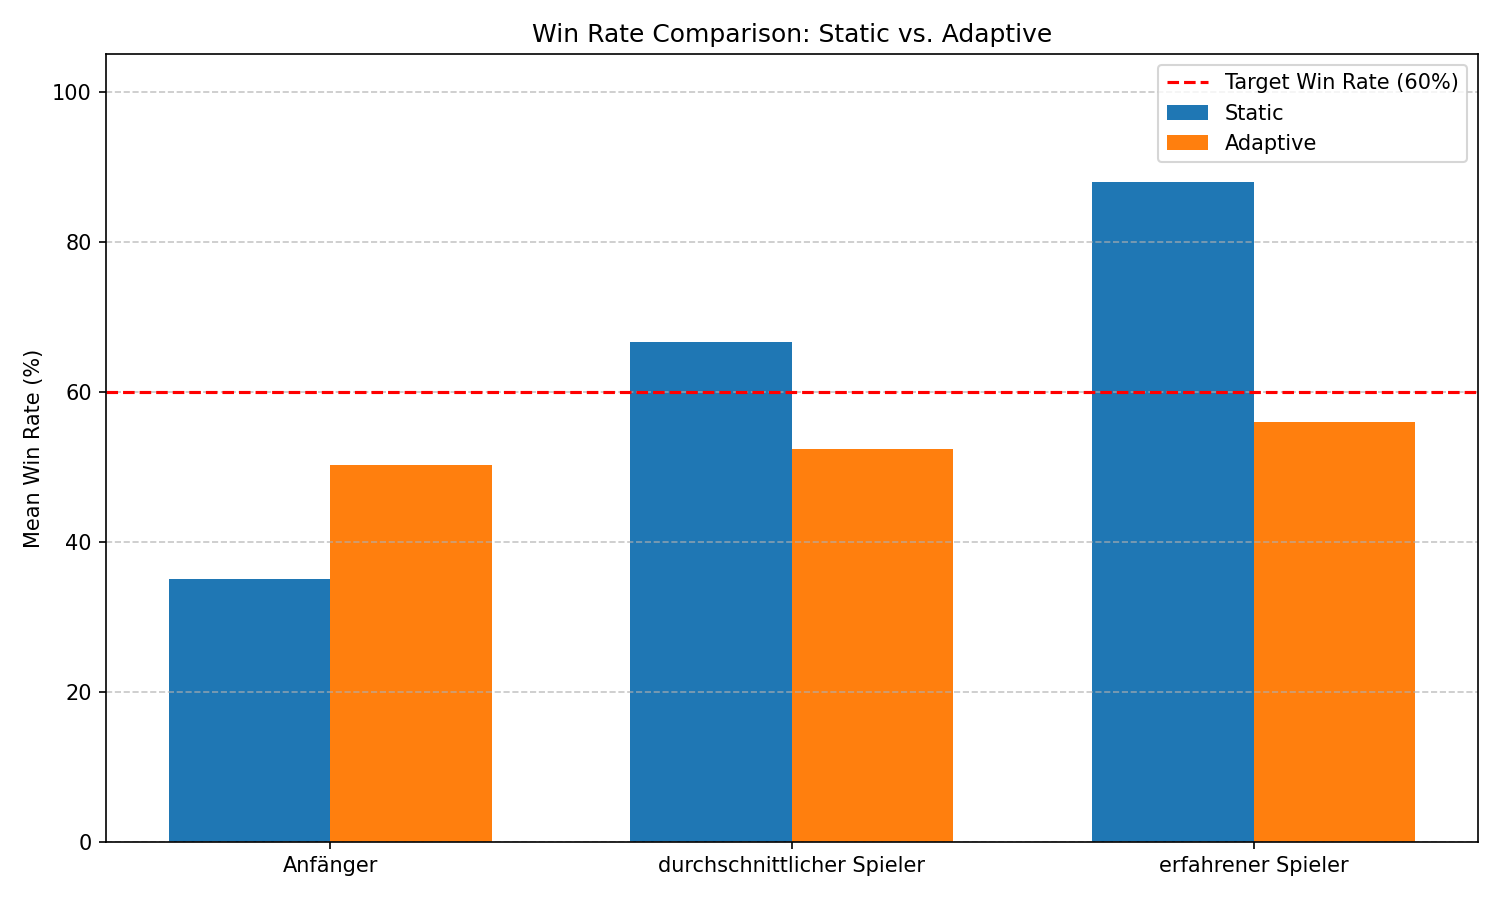
\includegraphics[width=\textwidth]{../results/figures/win_rate_comparison.png}
        \caption{Gewinnraten im Vergleich}
    \end{minipage}\hfill
    \begin{minipage}{0.48\textwidth}
        \centering
        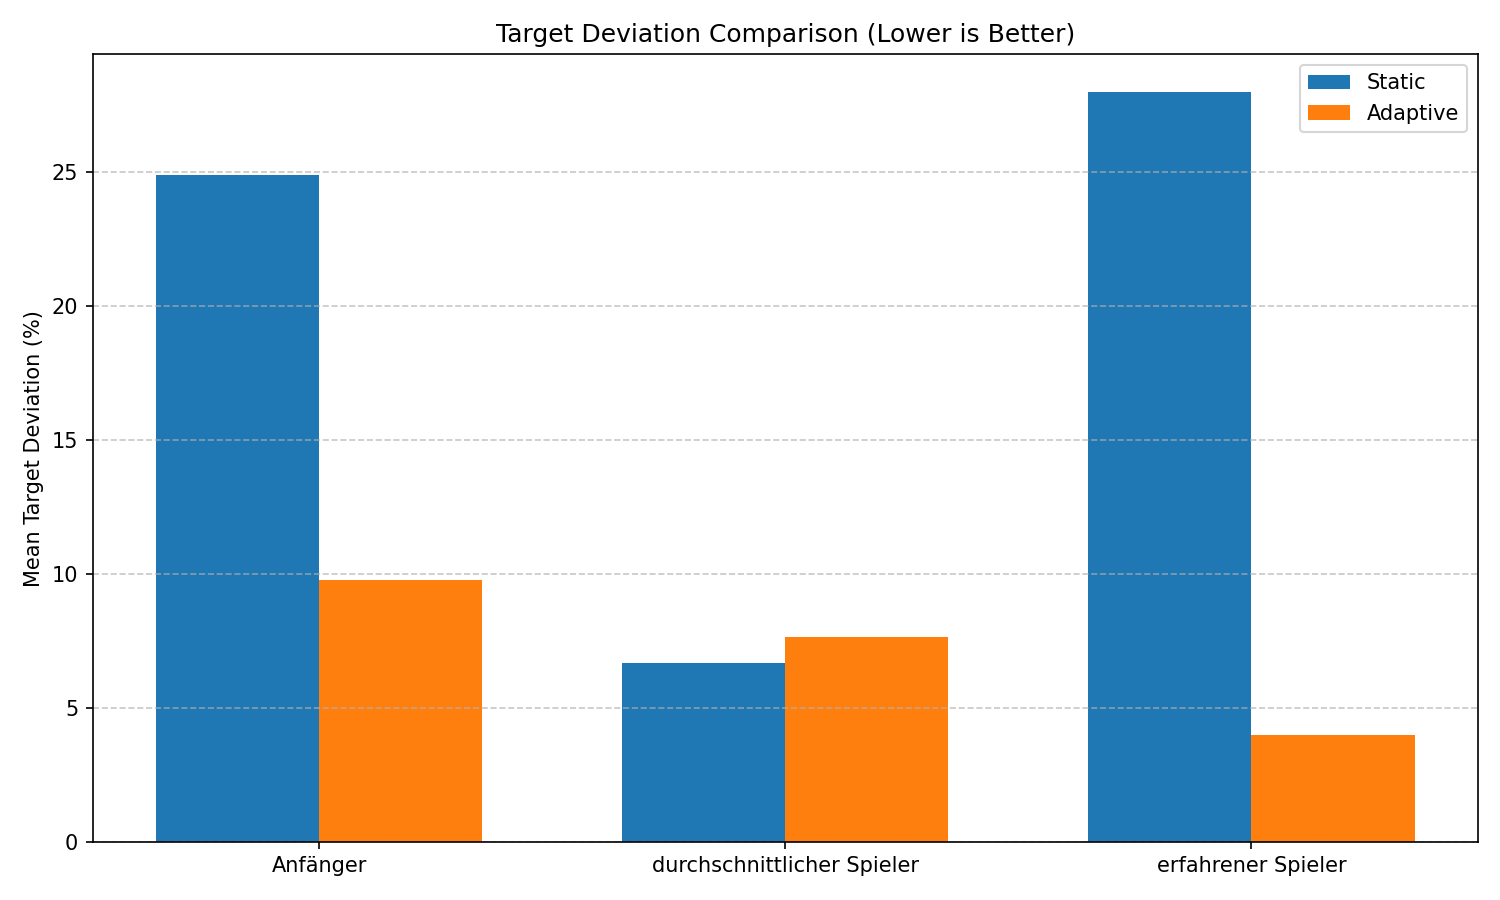
\includegraphics[width=\textwidth]{../results/figures/target_deviation.png}
        \caption{Abweichung von der Zielgewinnrate}
    \end{minipage}
\end{figure}

Die Ergebnisse verdeutlichen, dass das adaptive System nicht in jedem hypothetischen Fall pauschal überlegen ist. Wenn die initiale, statische Schwierigkeit bereits optimal auf das Leistungsniveau des Spielers abgestimmt ist, kann ein statisches System gleichwertige oder sogar marginal bessere Ergebnisse liefern. Die große Stärke der dynamischen Anpassung liegt vielmehr darin, extreme Über- oder Unterforderung zuverlässig zu erkennen und selbstständig zu korrigieren.

\section{Interaktive Live-Demo und Reaktionstest}

Zur greifbaren Demonstration des Systems wurde eine interaktive Konsolenanwendung entwickelt, welche über den Befehl \texttt{python main.py --interactive} gestartet werden kann. Dieser Modus bietet eine geführte Menüsteuerung, die zwischen der „Normalen Simulation“ und einem „Reaktionstest“ unterscheidet.

\textbf{Normale Simulation:}\\
In diesem Modus wählt der Nutzer eines der drei vordefinierten Profile (Anfänger, Durchschnitt, Experte) und definiert die Rundenanzahl sowie die Startschwierigkeit. Optional kann ein spezifischer Seed für reproduzierbare Durchläufe eingegeben werden; bleibt die Eingabe leer, wird ein zufälliger Seed generiert und für spätere Reproduktionen im Terminal angezeigt.
Während der Ausführung pausiert das System nach jeder Runde für circa 1,5 Sekunden. Die Ausgabe ist farblich formatiert: Ein Sieg wird in grün (\texttt{Player Won!}), eine Niederlage in rot (\texttt{Player Lost!}) dargestellt. Die Entscheidung des Agenten (z.\,B. \texttt{increase} aufgrund von drei Siegen in Folge) sowie der neue Schwierigkeitsgrad werden transparent in blau hervorgehoben.

\textbf{Reaktionstest:}\\
Der Reaktionstest erweitert die Demo um eine spielerische Profilgenerierung. Das System misst die Reaktionszeit des Nutzers auf ein im Terminal erscheinendes Signal. Der Test erfordert standardmäßig 5 Messungen, wobei Eingaben unter 80 ms als Frühstarts abgelehnt und wiederholt werden.
Aus den gültigen Messungen wird der Median gebildet und über eine lineare Interpolation in einen normierten Reaktionswert ($0,0$ bis $1,0$) überführt. Dieser gemessene Wert wird als \texttt{reaction\_speed} in ein neues, personalisiertes Profil übernommen. Die restlichen Parameter des Profils verbleiben auf dem Niveau eines durchschnittlichen Spielers. Anschließend startet die adaptive Demo automatisch mit diesem personalisierten Profil. Die im Terminal angezeigten Kategorien (\texttt{expert}, \texttt{average}, \texttt{beginner}) dienen rein als visuelles Feedback für die Demo und stellen keine wissenschaftlich fundierte Leistungsdiagnostik dar.

\section{Qualitätssicherung und Reproduzierbarkeit}

Die strukturelle Integrität des Quellcodes und der Logik wird durch eine umfassende Testsuite unter Verwendung des \texttt{pytest}-Frameworks gewährleistet. Der aktuelle Entwicklungsstand weist \textbf{118 bestandene automatisierte Tests} auf.

Diese Tests decken ein breites Spektrum ab:
\begin{itemize}
    \item \textbf{Kernlogik:} Validierung der Spielerprofile, strikte Einhaltung der Simulationsgrenzen und korrekte Konvertierung des Schwierigkeitsgrades in Spielparameter.
    \item \textbf{Agentenentscheidungen:} Systematische Prüfung aller Entscheidungsregeln des adaptiven Agenten unter verschiedenen Randbedingungen.
    \item \textbf{Experimentablauf:} Überprüfung der statischen und adaptiven Testreihen sowie der korrekten Generierung des CSV-Exports.
    \item \textbf{Reaktionstest \& Interaktion:} Tests zur Medianberechnung, Clamping von Reaktionswerten, Ablehnung unzulässiger Messungen unter 80 ms und Validierung von Nutzereingaben. Um Verzögerungen in der Testausführung zu vermeiden, werden \texttt{input} und \texttt{sleep} für die interaktiven Tests gemockt.
\end{itemize}

Ein zentraler Aspekt der Qualitätssicherung ist die \textbf{Reproduzierbarkeit}. Die wissenschaftlichen Experimente nutzen ausschließlich feste Seeds. Innerhalb der Simulation wird für jede Runde ein deterministischer Folgeseed generiert (Basis-Seed $+$ Rundennummer $- 1$). Dadurch ist garantiert, dass bei gleichen Startparametern die Simulation und die erzeugten CSV-Dateien exakt reproduzierbar sind. Lediglich die vom Menschen im Reaktionstest produzierten Messwerte unterliegen natürlichen Varianzen und entziehen sich einer deterministischen Reproduktion.

\section{Grenzen, Fazit und Ausblick}

\subsection{Grenzen des Modells}
Die Aussagekraft der Ergebnisse ist an den Rahmen der Abstraktion gebunden. Das Projekt verwendet eine vereinfachte, probabilistische Simulation anstelle einer hochauflösenden Game Engine und operiert mit synthetischen Spielerprofilen anstatt echter Telemetriedaten. Der Agent stützt sich auf feste Regeln und ist nicht in der Lage, eigenständig zu lernen. Zudem ist die Gewinnrate als alleiniger Proxy für Spielbalance unvollständig. Reale Faktoren wie das Gefühl der Fairness, Pacing oder visuelles Feedback bleiben unberücksichtigt. Schließlich ist die Reaktionsmessung im Terminal abhängig von Hardware-Latenzen und stellt kein präzises Messinstrument dar.

\subsection{Fazit}
Bezugnehmend auf die Forschungsfrage lässt sich schlussfolgern: Ein adaptiver Schwierigkeitsagent kann eine ausgewogenere Spielerfahrung erzeugen als ein statisches System, sofern die anfängliche, statische Schwierigkeit nicht zum Leistungsniveau des Spielers passt. Insbesondere bei Anfängern und Experten korrigiert das adaptive System signifikante Über- oder Unterforderung zuverlässig und führt die Gewinnrate näher an das definierte Ziel. Ist der statische Schwierigkeitsgrad jedoch initial exakt kalibriert, bietet das adaptive System keinen quantitativen Vorteil. Das Projekt belegt somit erfolgreich die grundlegende Funktionalität und den Nutzen von regelbasierter dynamischer Schwierigkeitsanpassung.

\subsection{Ausblick}
Zukünftige Arbeiten könnten die Validität der Ergebnisse erhöhen, indem der Agent in eine reale Game Engine (z.\,B. Godot oder Unity) integriert wird, um echte Telemetriedaten zu verarbeiten. Das Simulationsmodell könnte um Parameter wie gegnerische KI-Komplexität oder Ressourcenmanagement erweitert werden. Eine dynamische, personalisierte Anpassung der Zielgewinnrate, abhängig vom Spielerverhalten, könnte die Benutzererfahrung weiter individualisieren. Schließlich wäre der Einsatz und direkte Vergleich eines lernenden Agenten (z.\,B. Reinforcement Learning) mit dem hier entwickelten regelbasierten Ansatz ein vielversprechendes Forschungsvorhaben.

\end{document}
